%\documentclass[11pt]{article}
\documentclass[•]{oblivoir}

\usepackage{graphicx}
\usepackage{subfig}
\usepackage{tabu}
\usepackage{lipsum}
\usepackage{xcolor}
\usepackage{multirow}
\definecolor{Plum}{rgb}{0.56, 0.27, 0.52}
\definecolor{OliveDrab}{rgb}{0.42, 0.56, 0.14}
\definecolor{RedViolet}{rgb}{0.78, 0.08, 0.52}
\definecolor{Brown}{rgb}{0.65, 0.16, 0.16}
\definecolor{Blue}{rgb}{0, 0, 1}

%\grapicspath{{./pictures01}{./picture02}}
\graphicspath{{./pictures/}}

\begin{document}
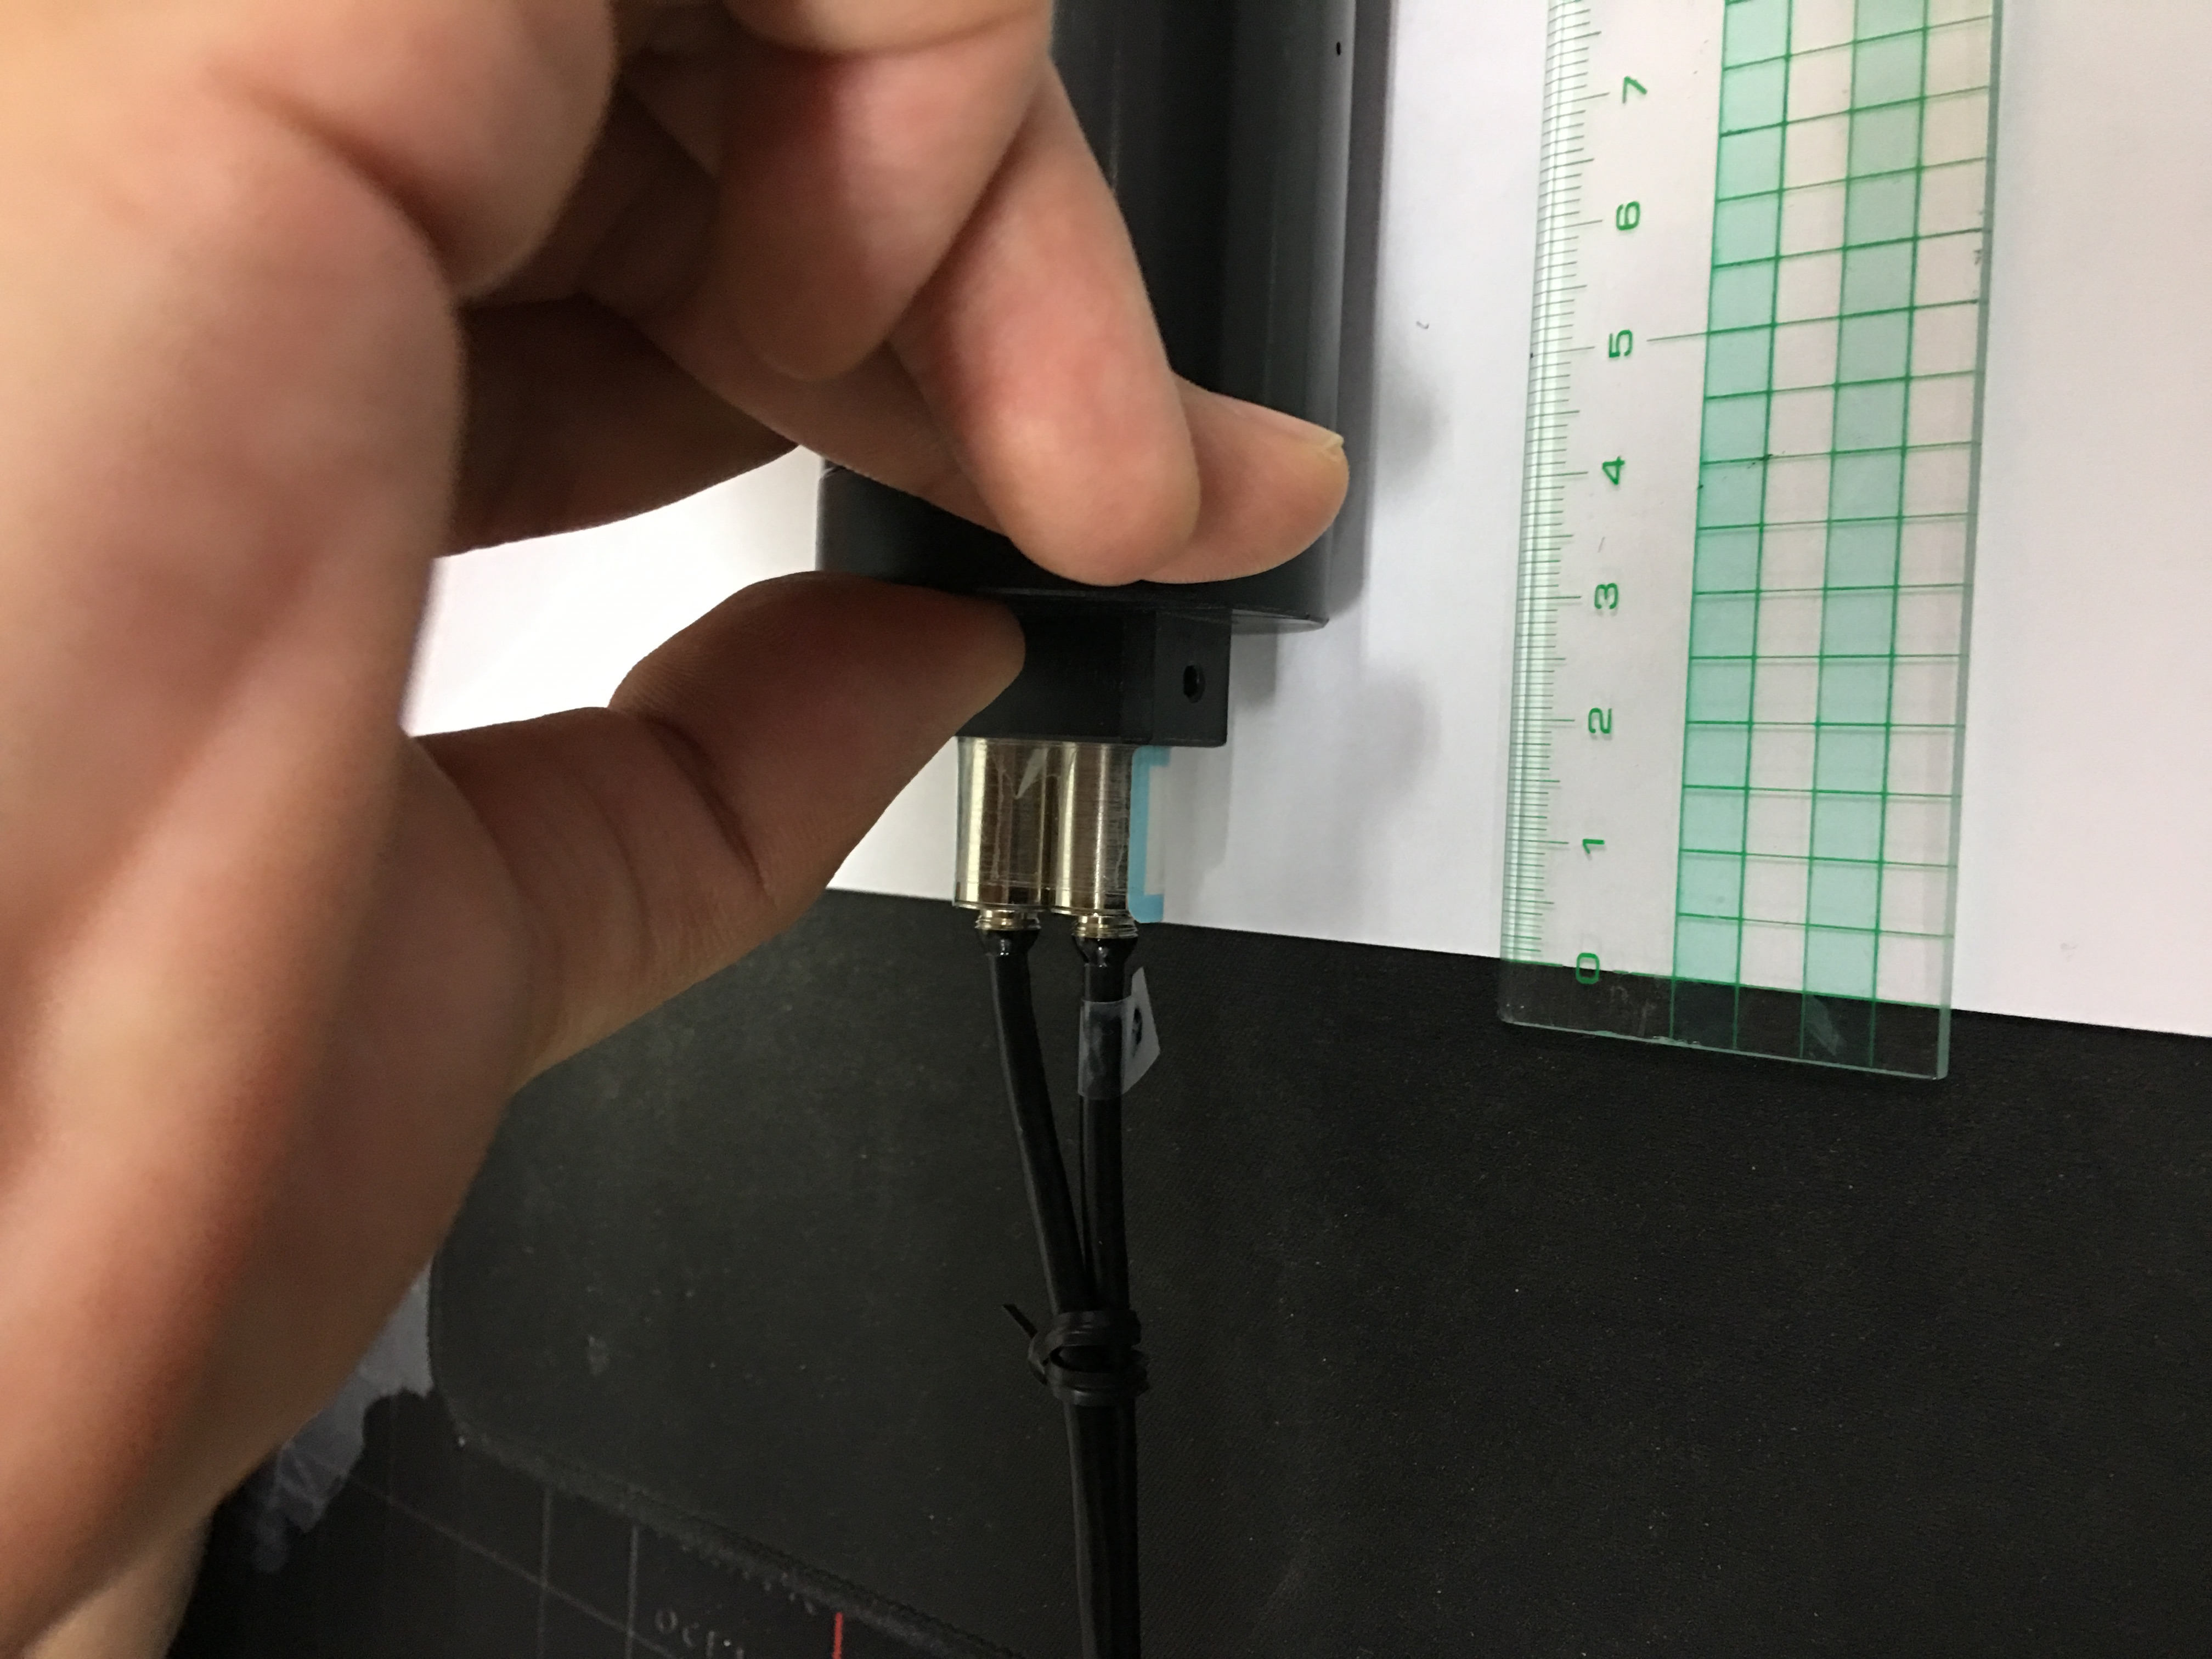
\includegraphics[width=0.8\textwidth]{img01.jpg}
%\includegraphics[width=0.8\textwidth, page={3}]{RedVelvet.pdf}

\begin{center}
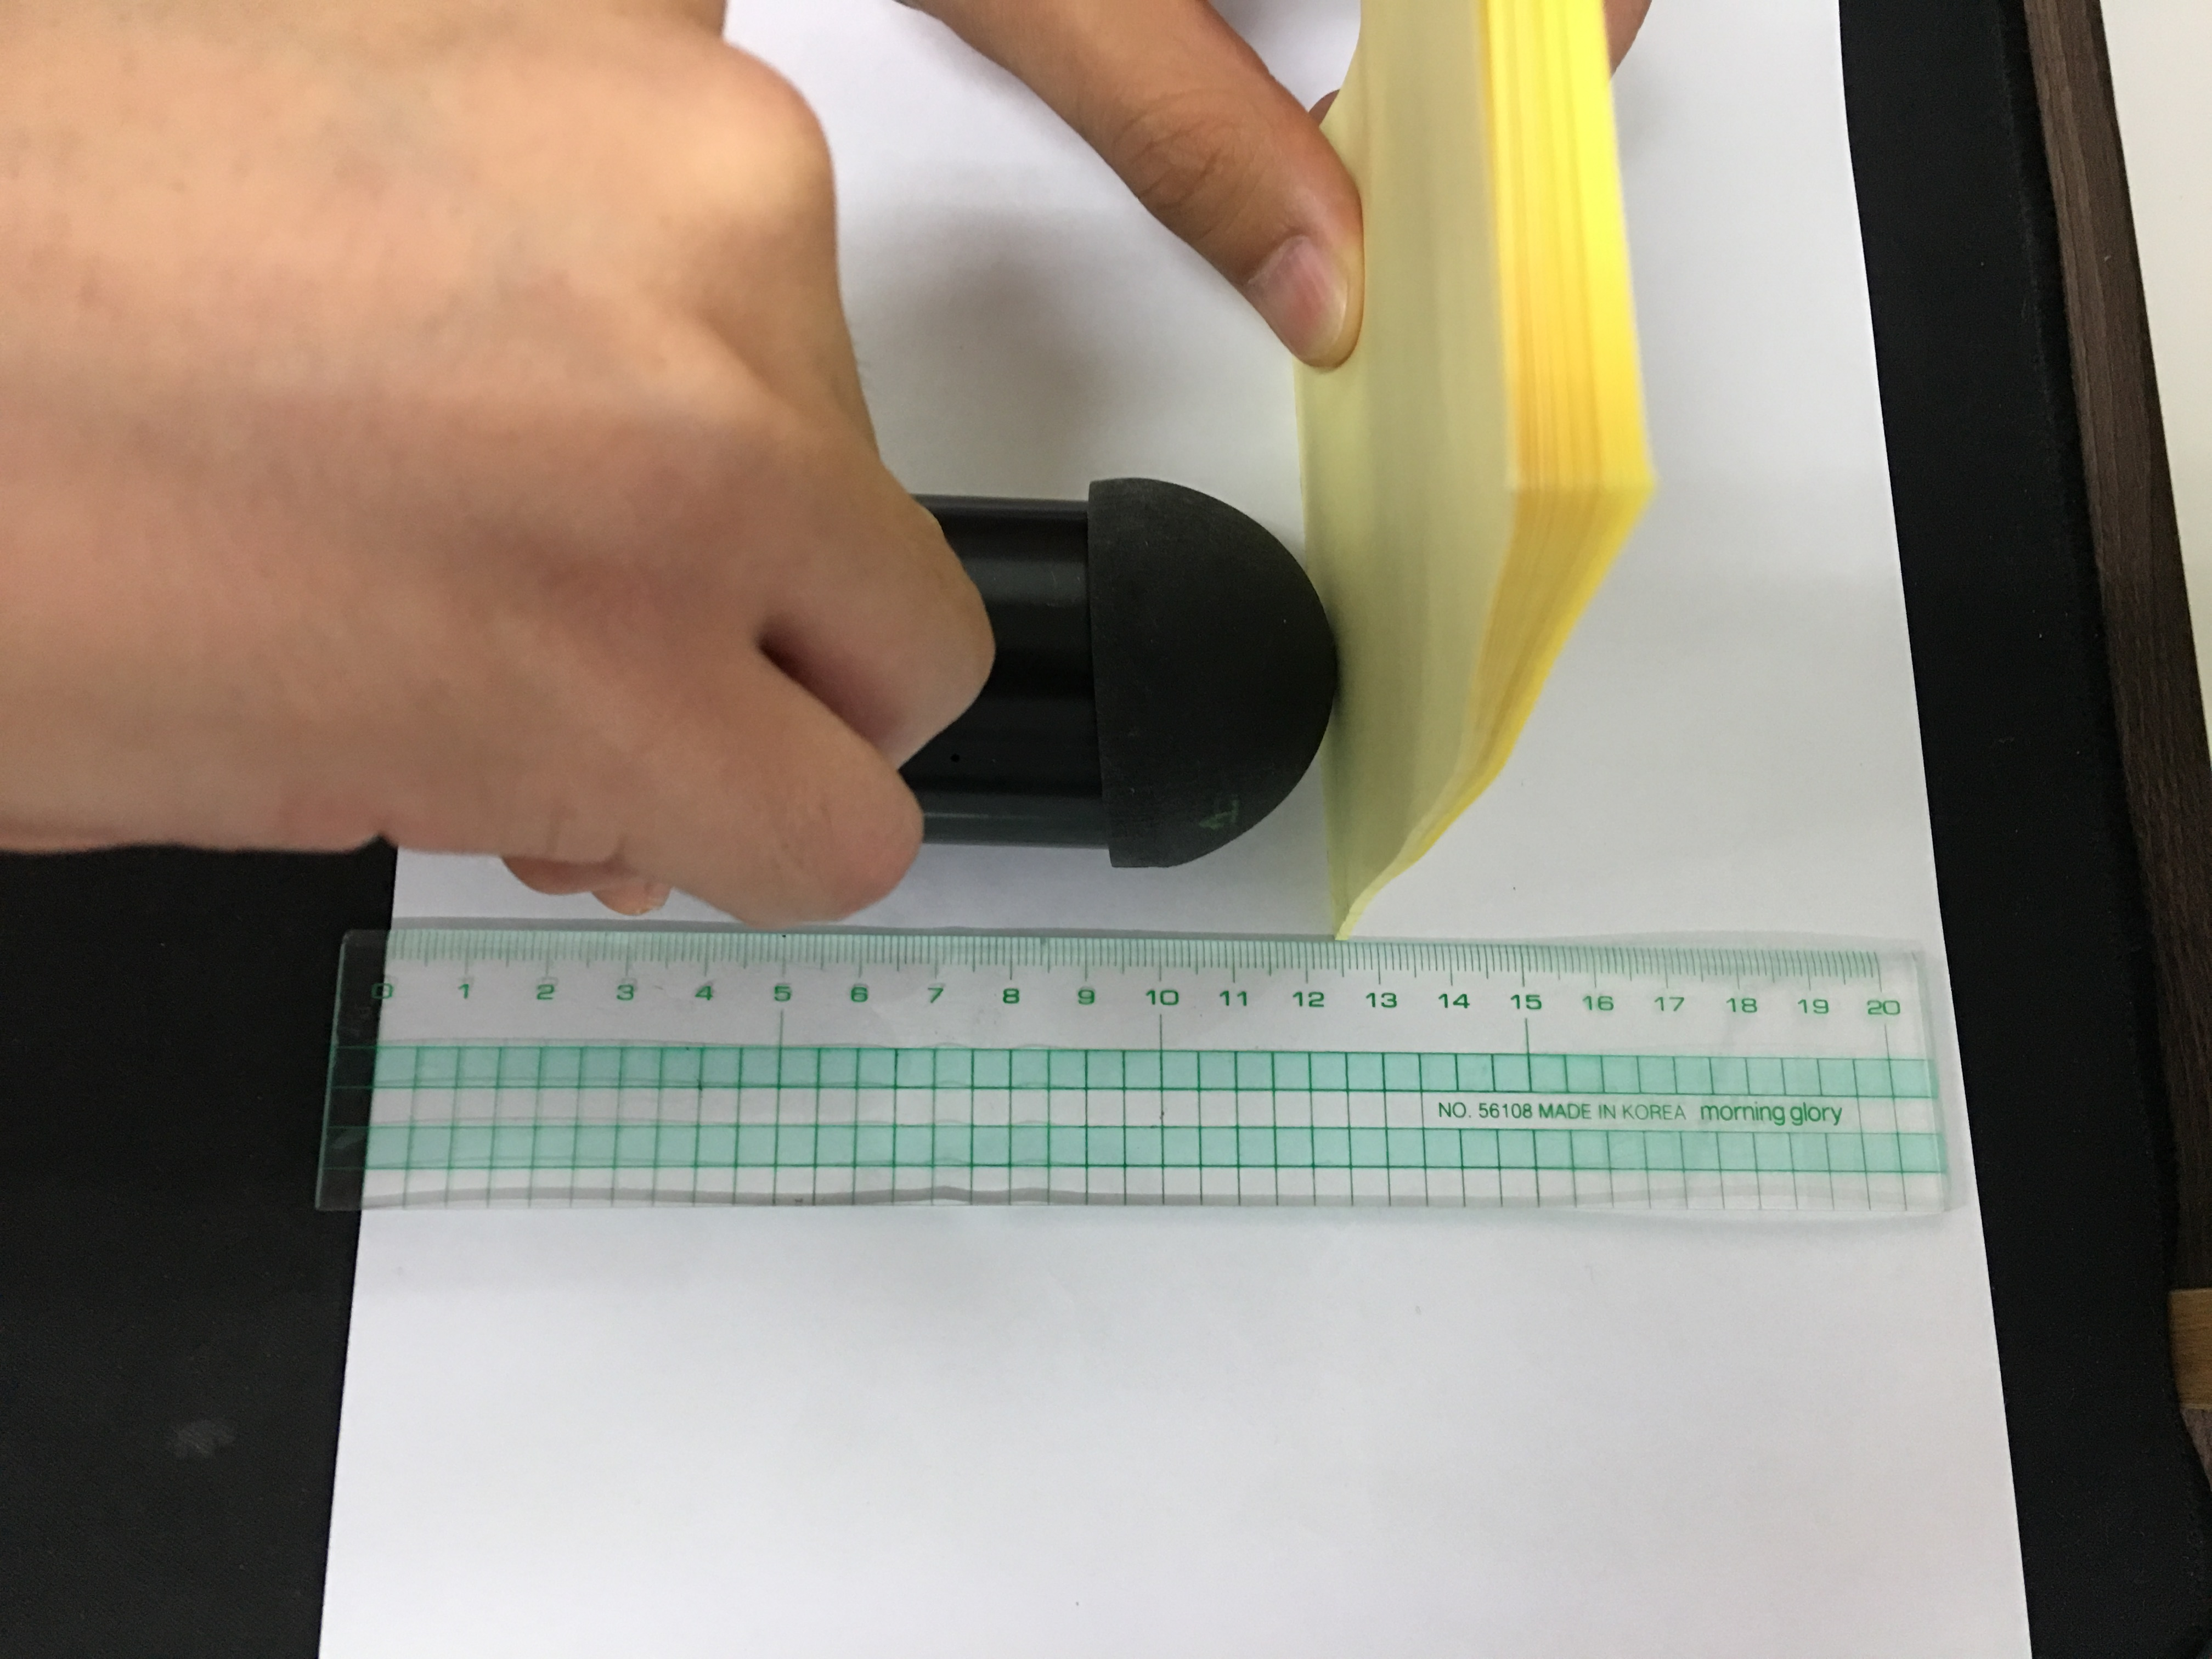
\includegraphics[width=0.8\textwidth]{img02}
\end{center}

\begin{figure}[t]
\centering
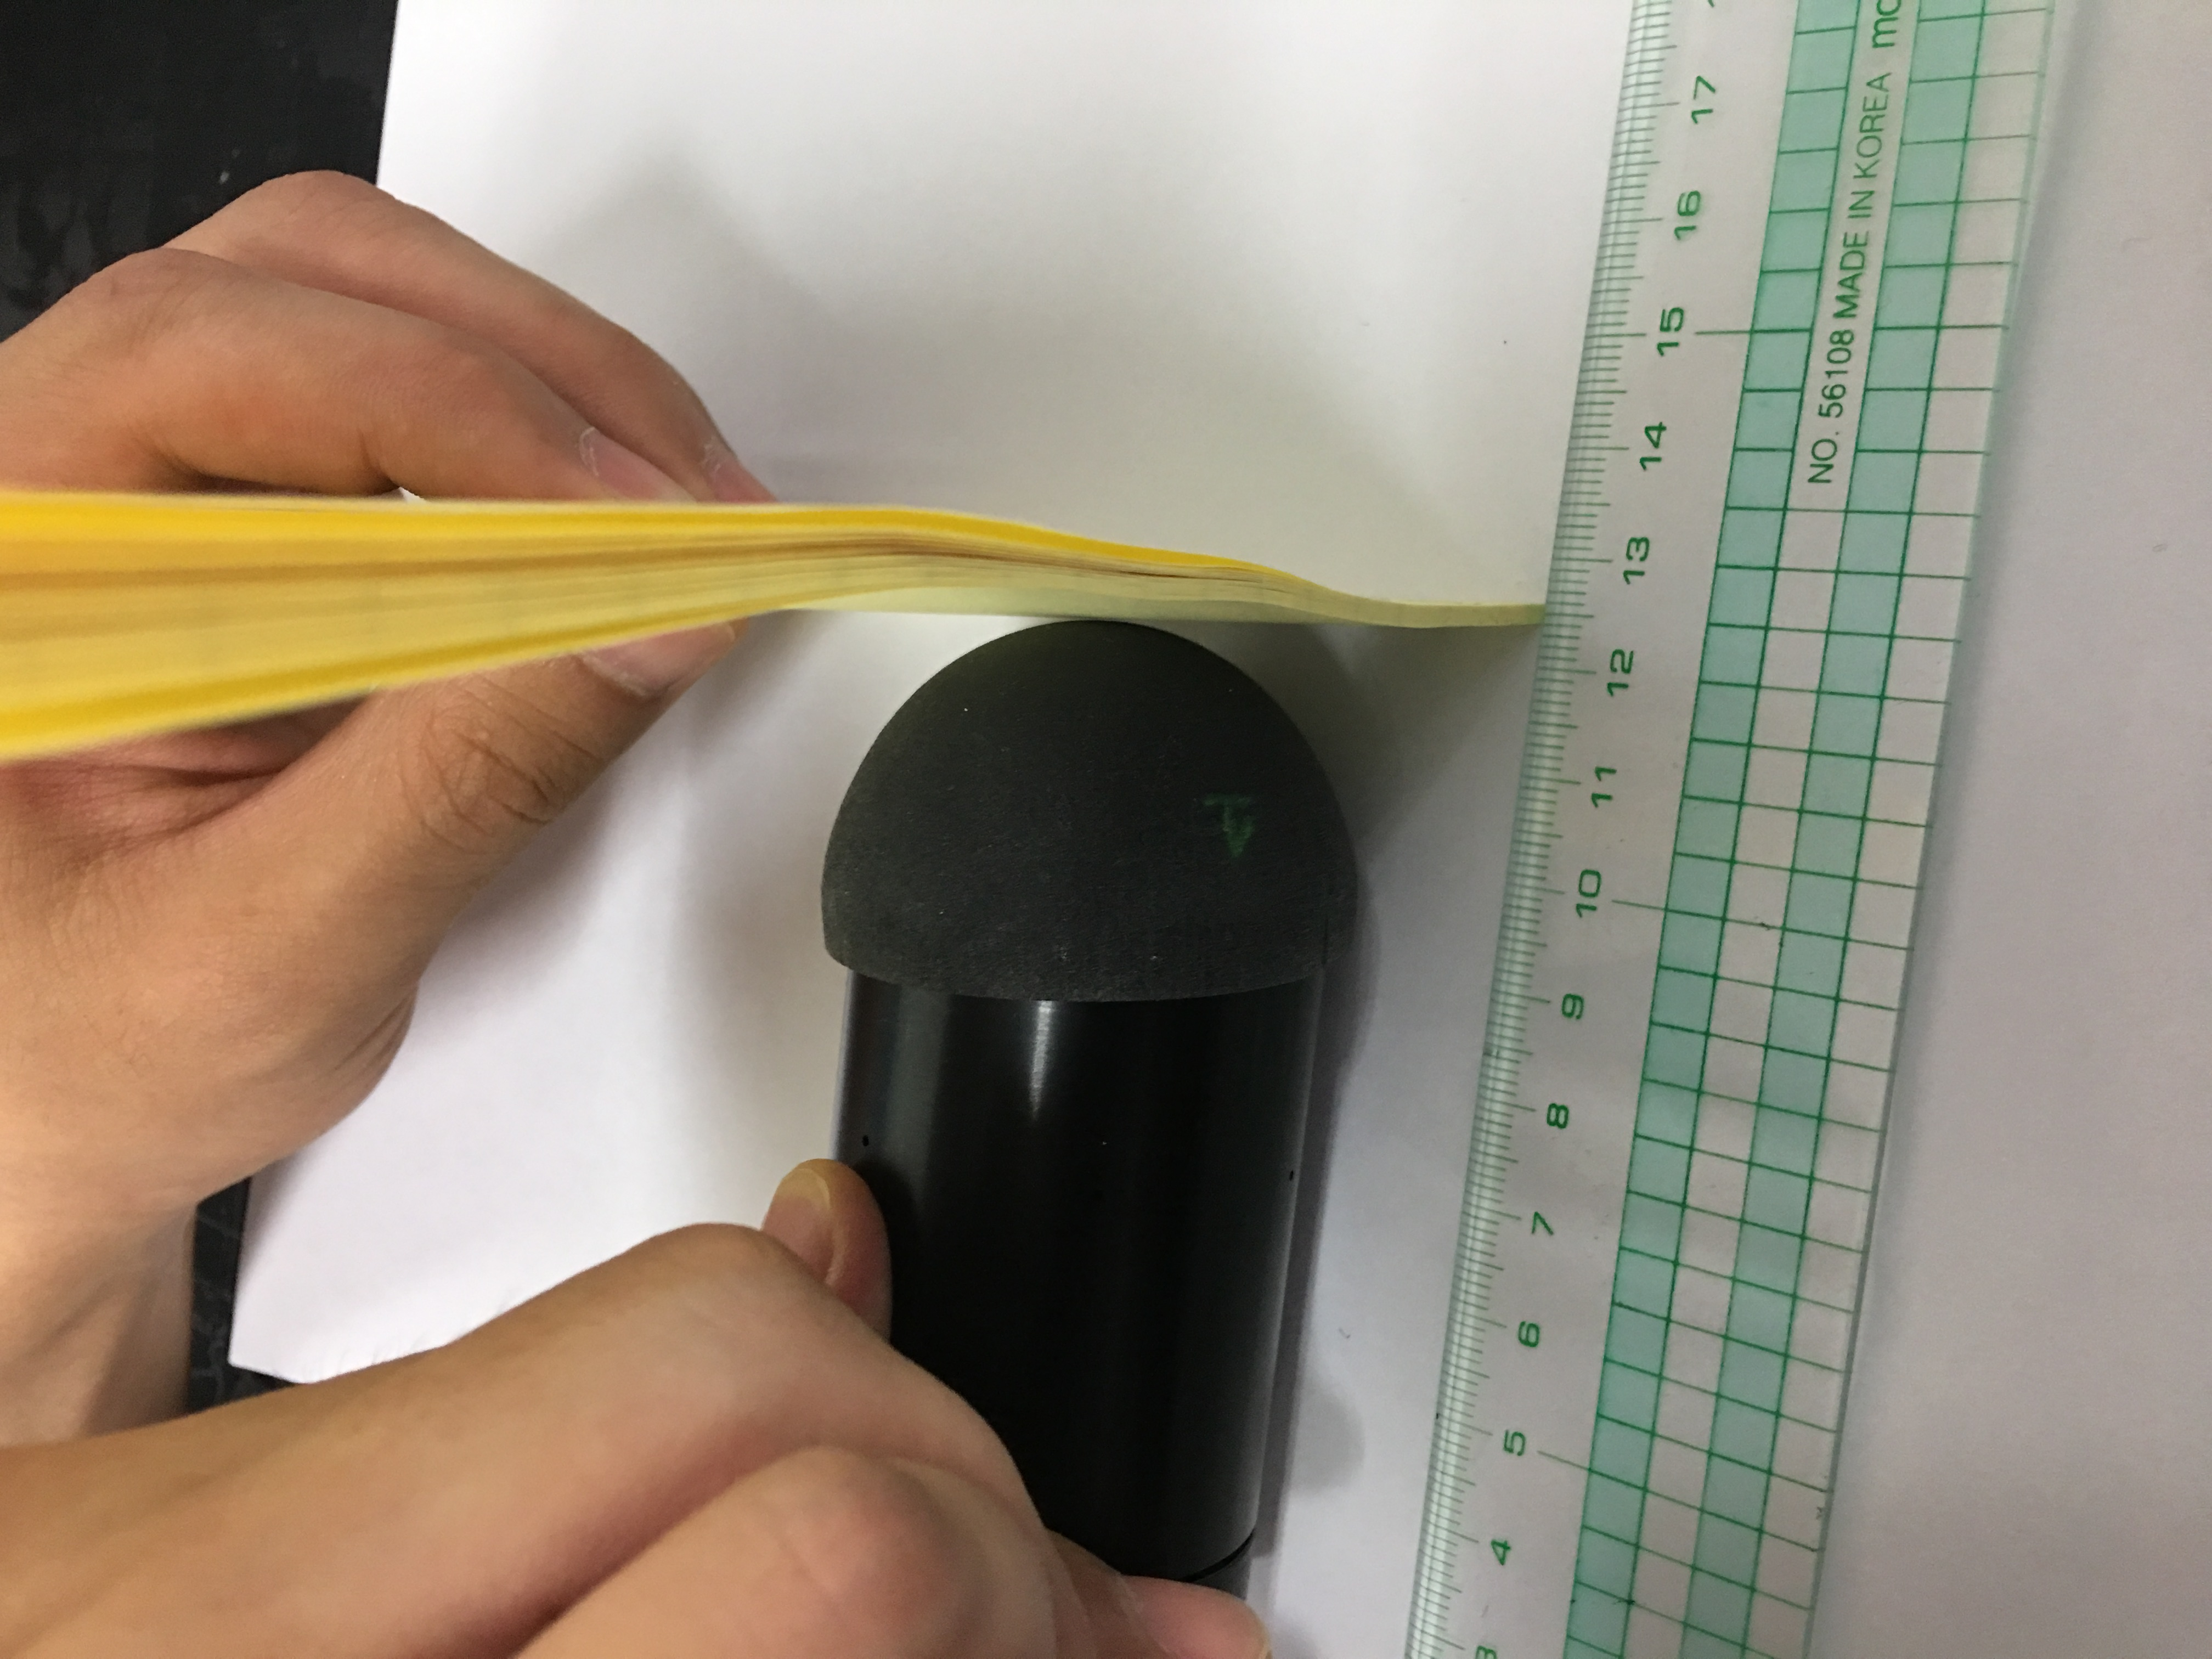
\includegraphics[width=0.8\textwidth]{img03}
\caption{촉각센서 이미지}\label{fig:1}
\end{figure}

\lipsum

그림 \ref{fig:1}\를 참고하라.

\begin{figure}
\centering
\subfloat[img01]
{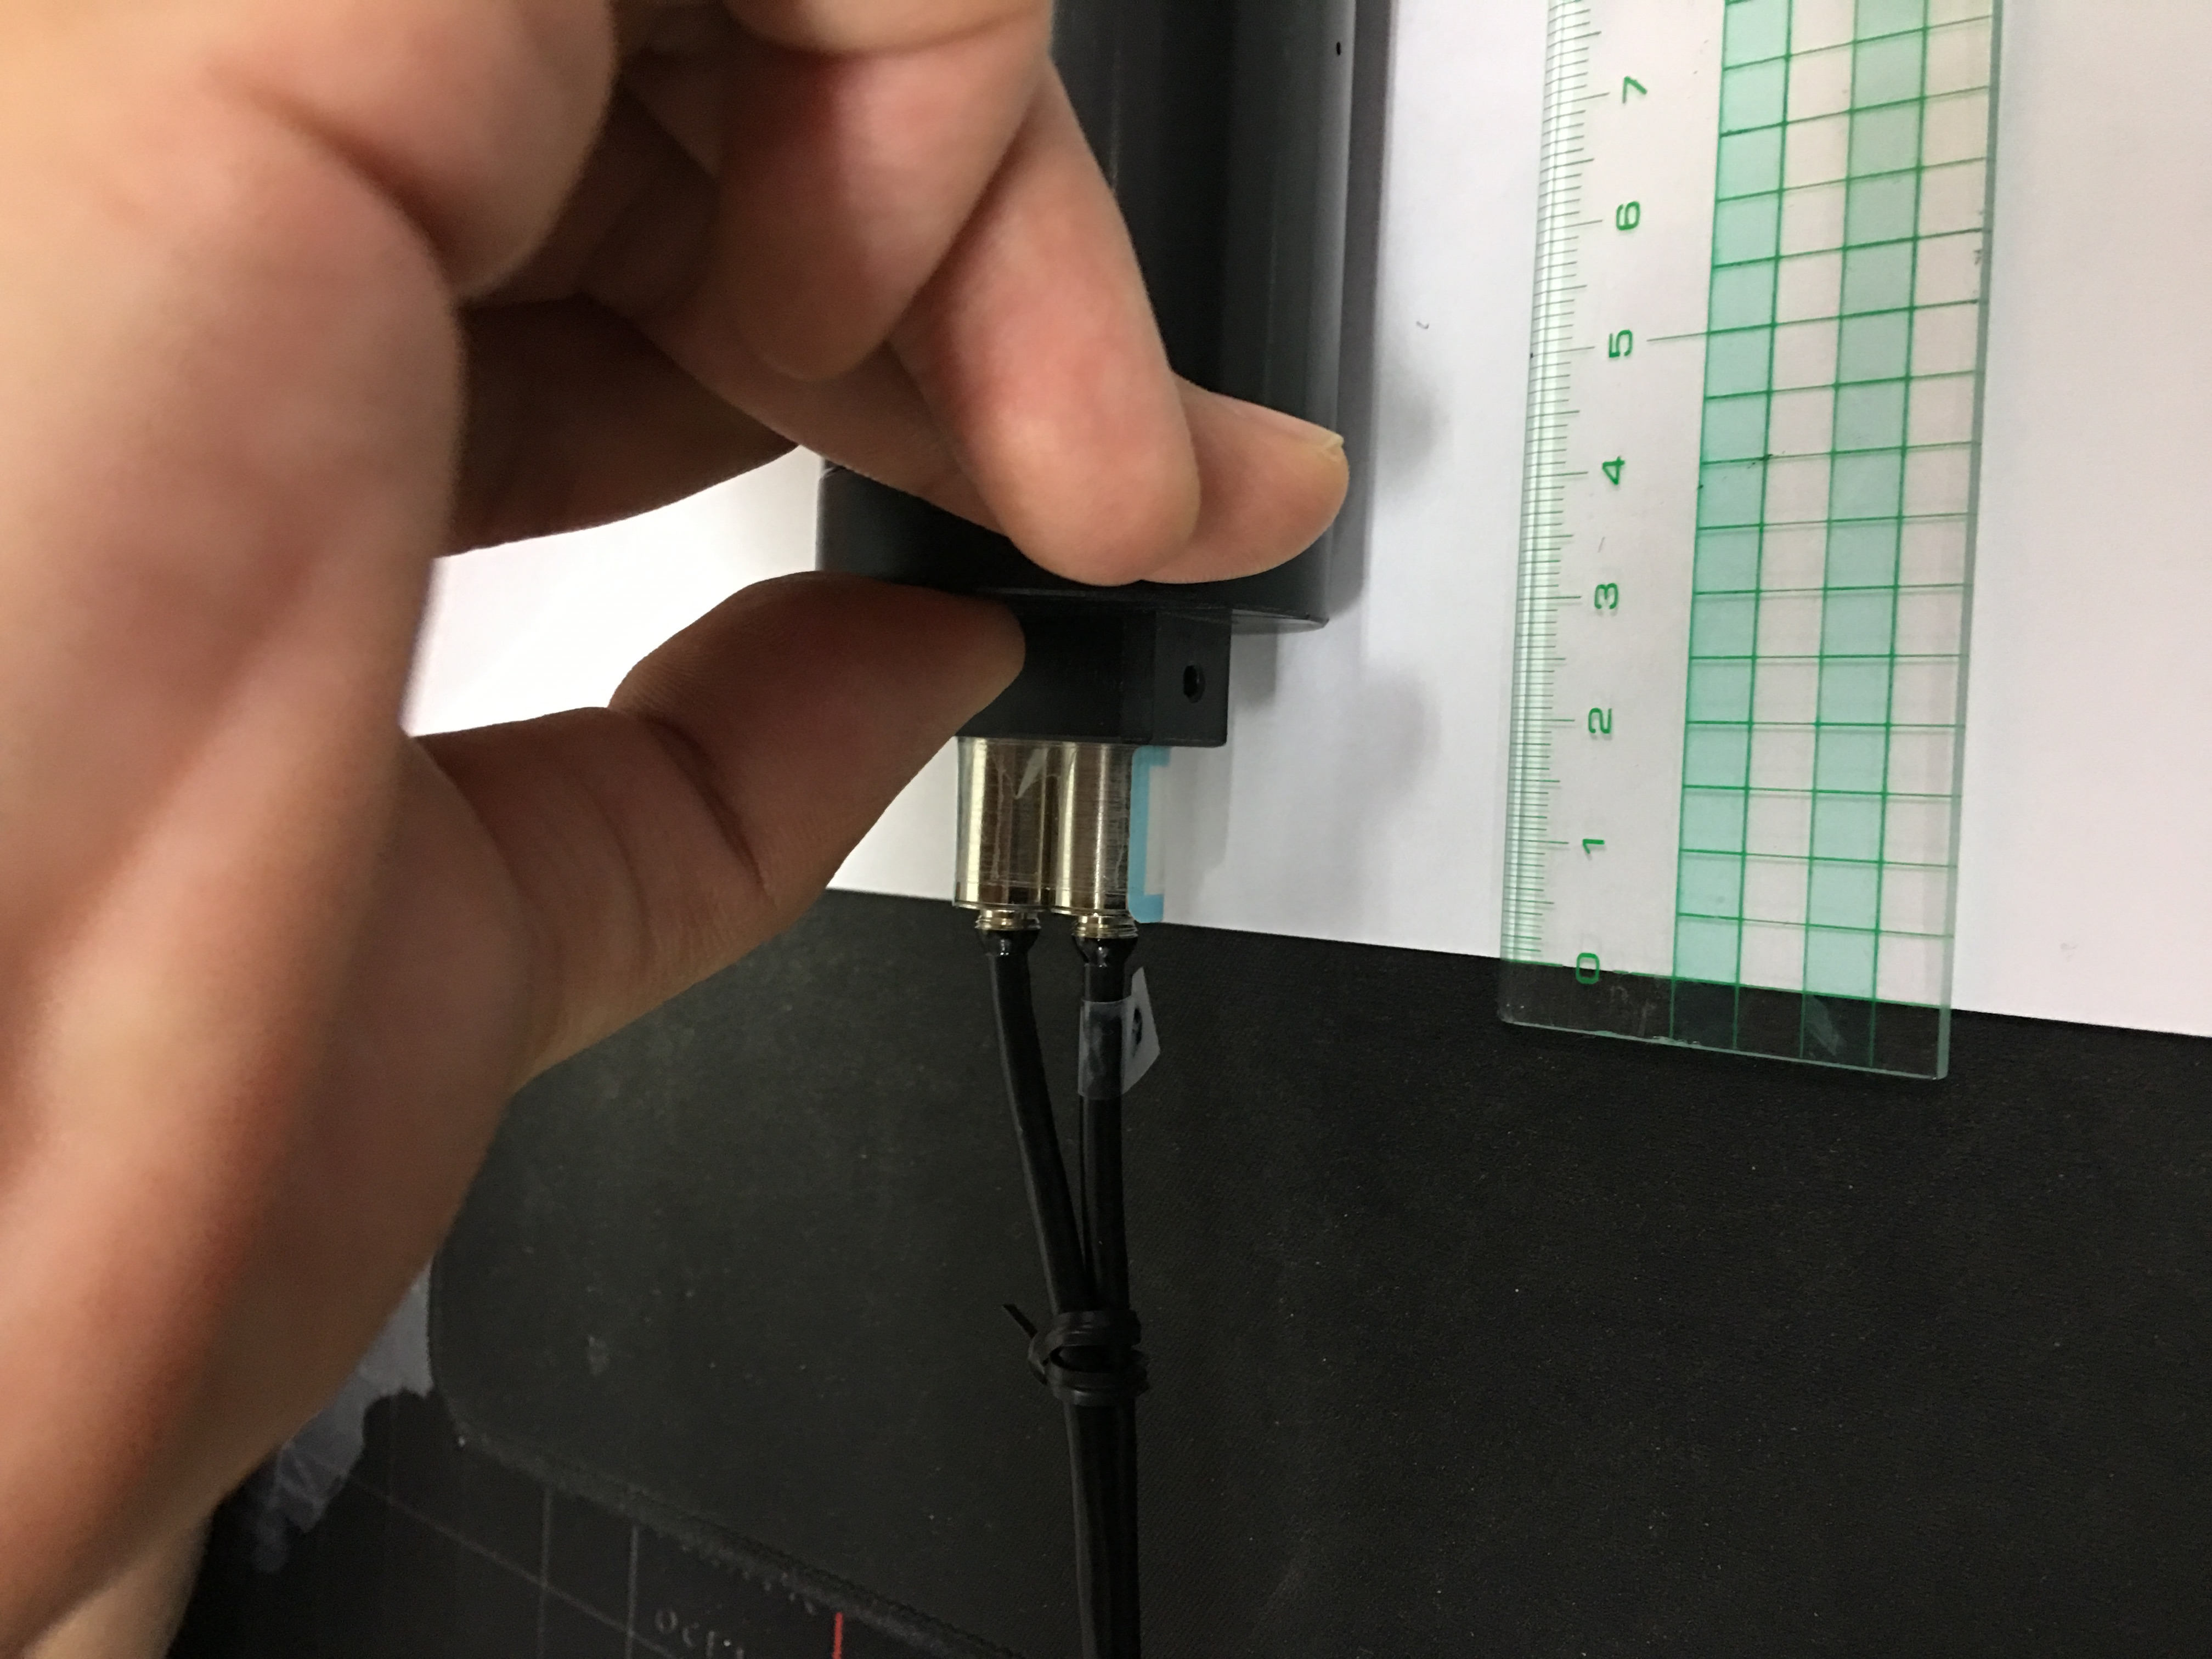
\includegraphics[width=0.3\textwidth]{img01.jpg}}
\quad
\subfloat[img02]
{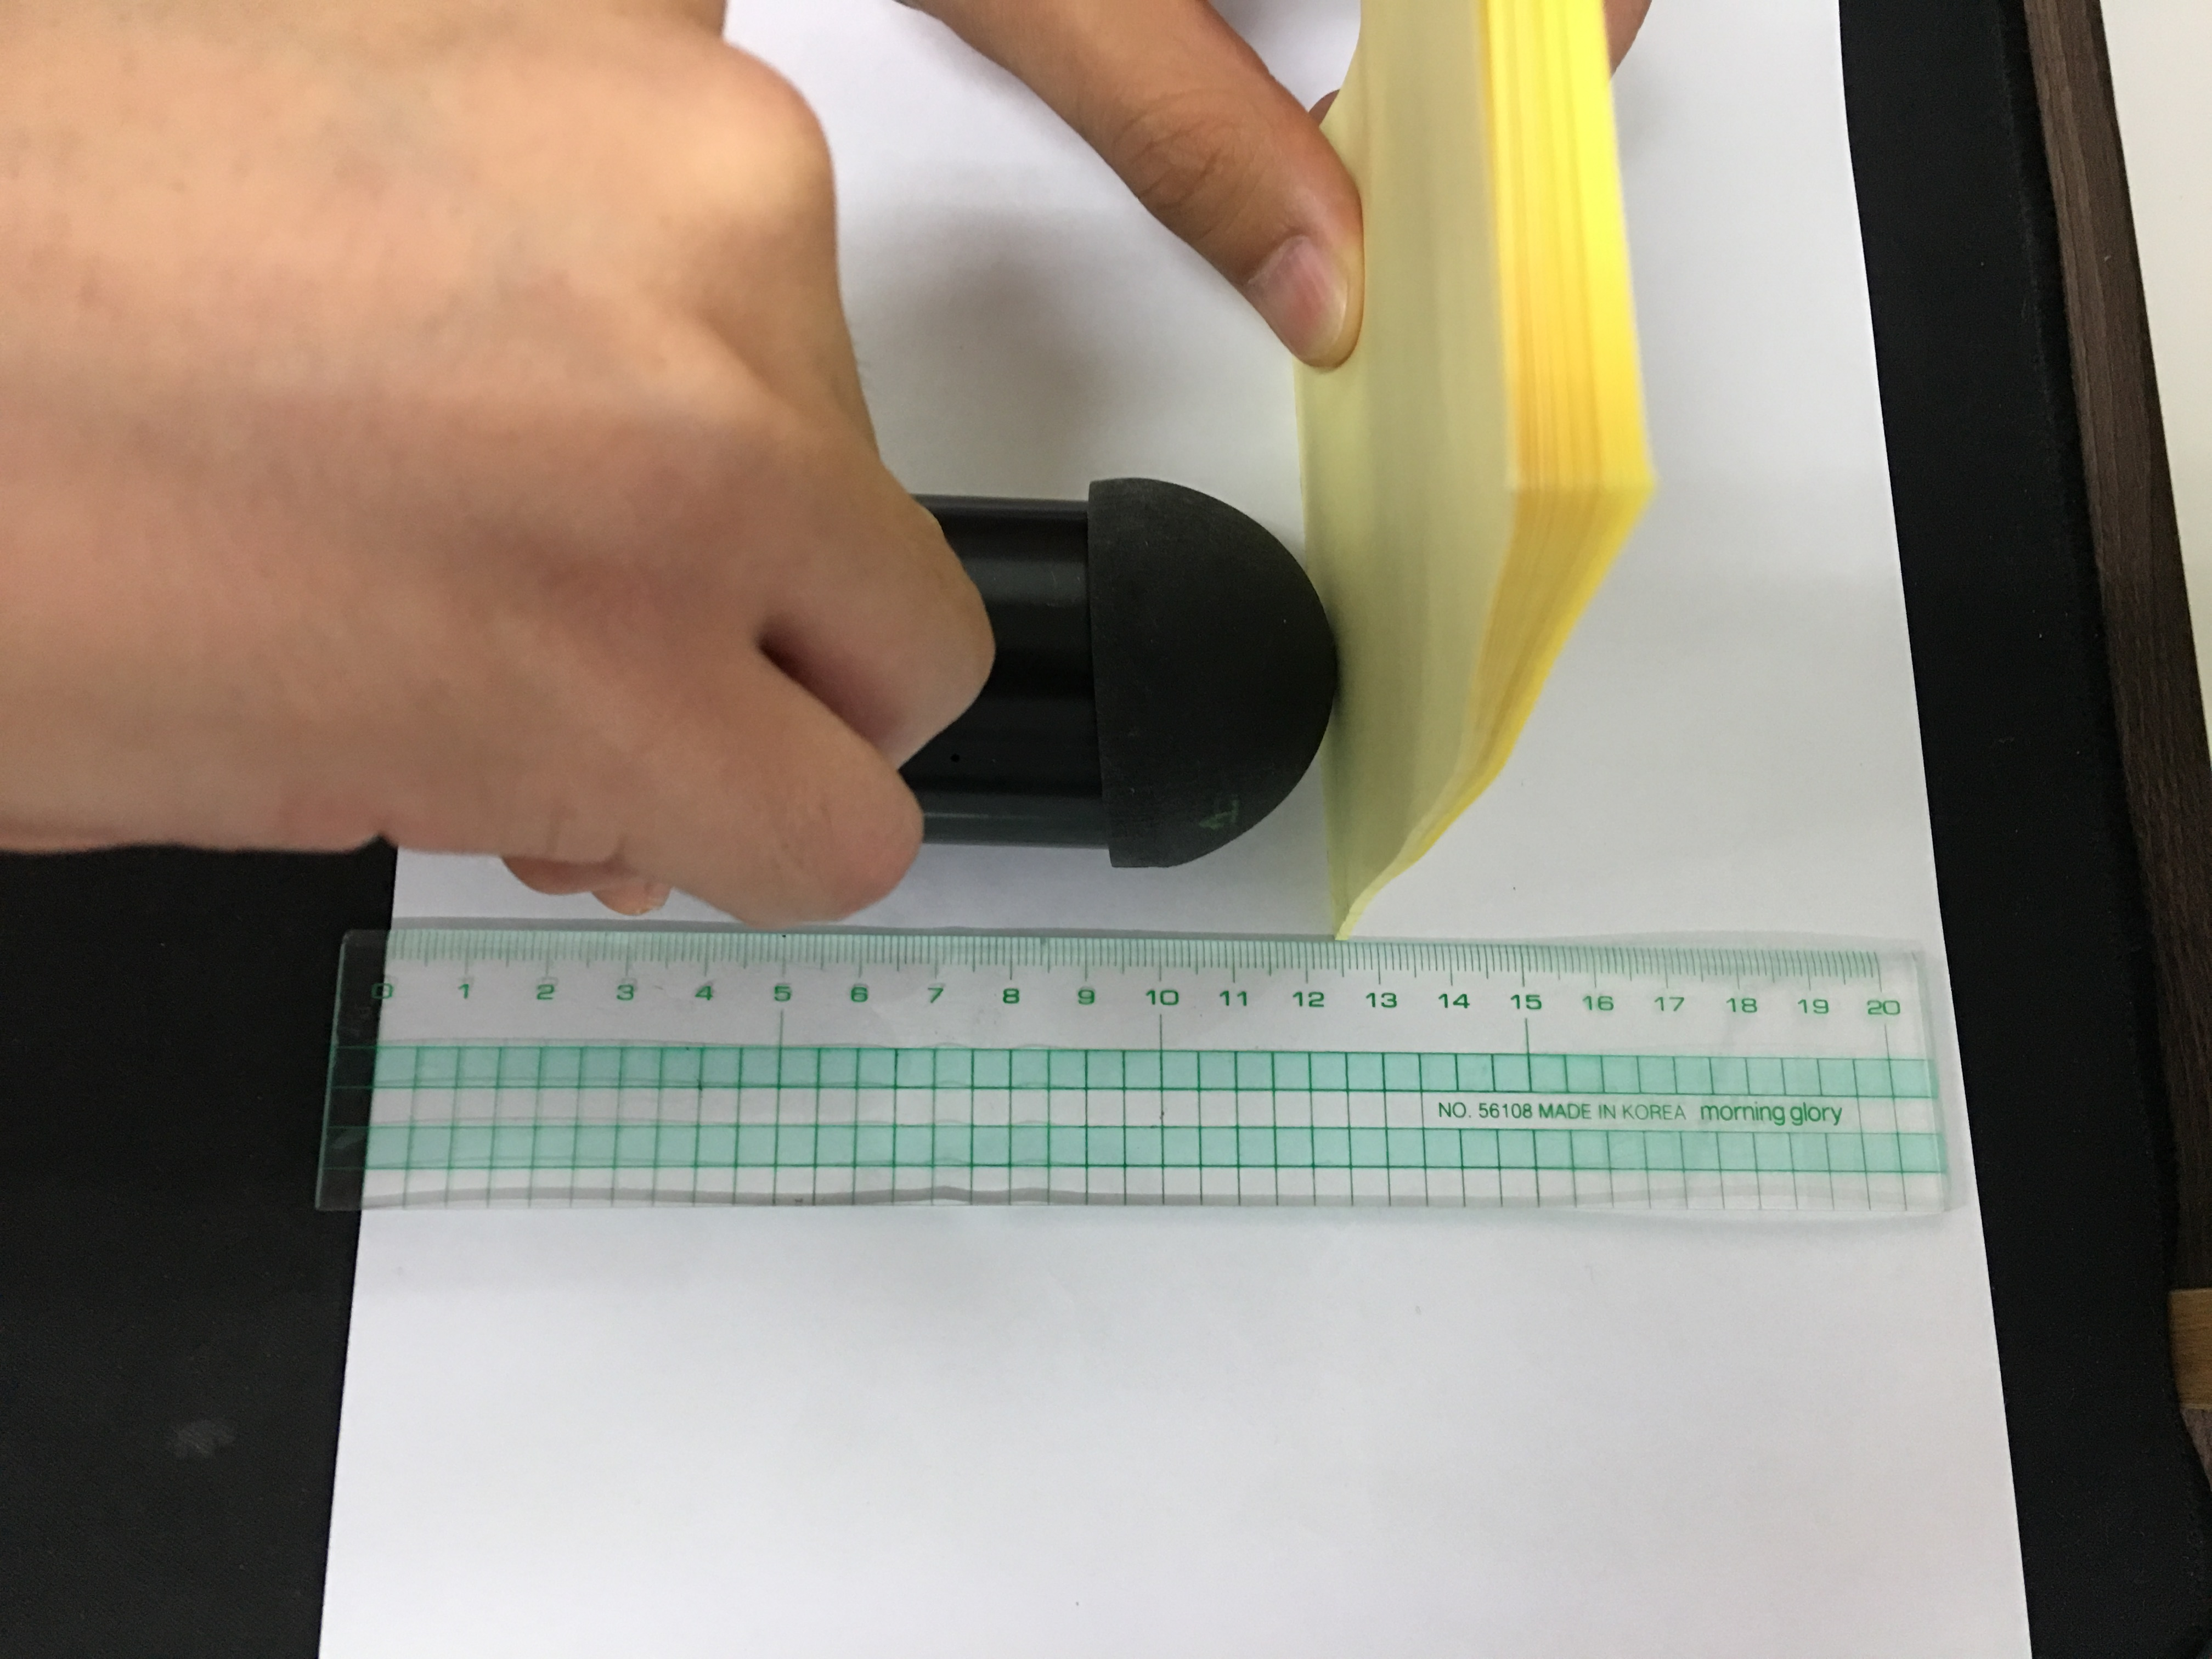
\includegraphics[width=0.3\textwidth]{img02.jpg}}
\quad
\subfloat[img03]
{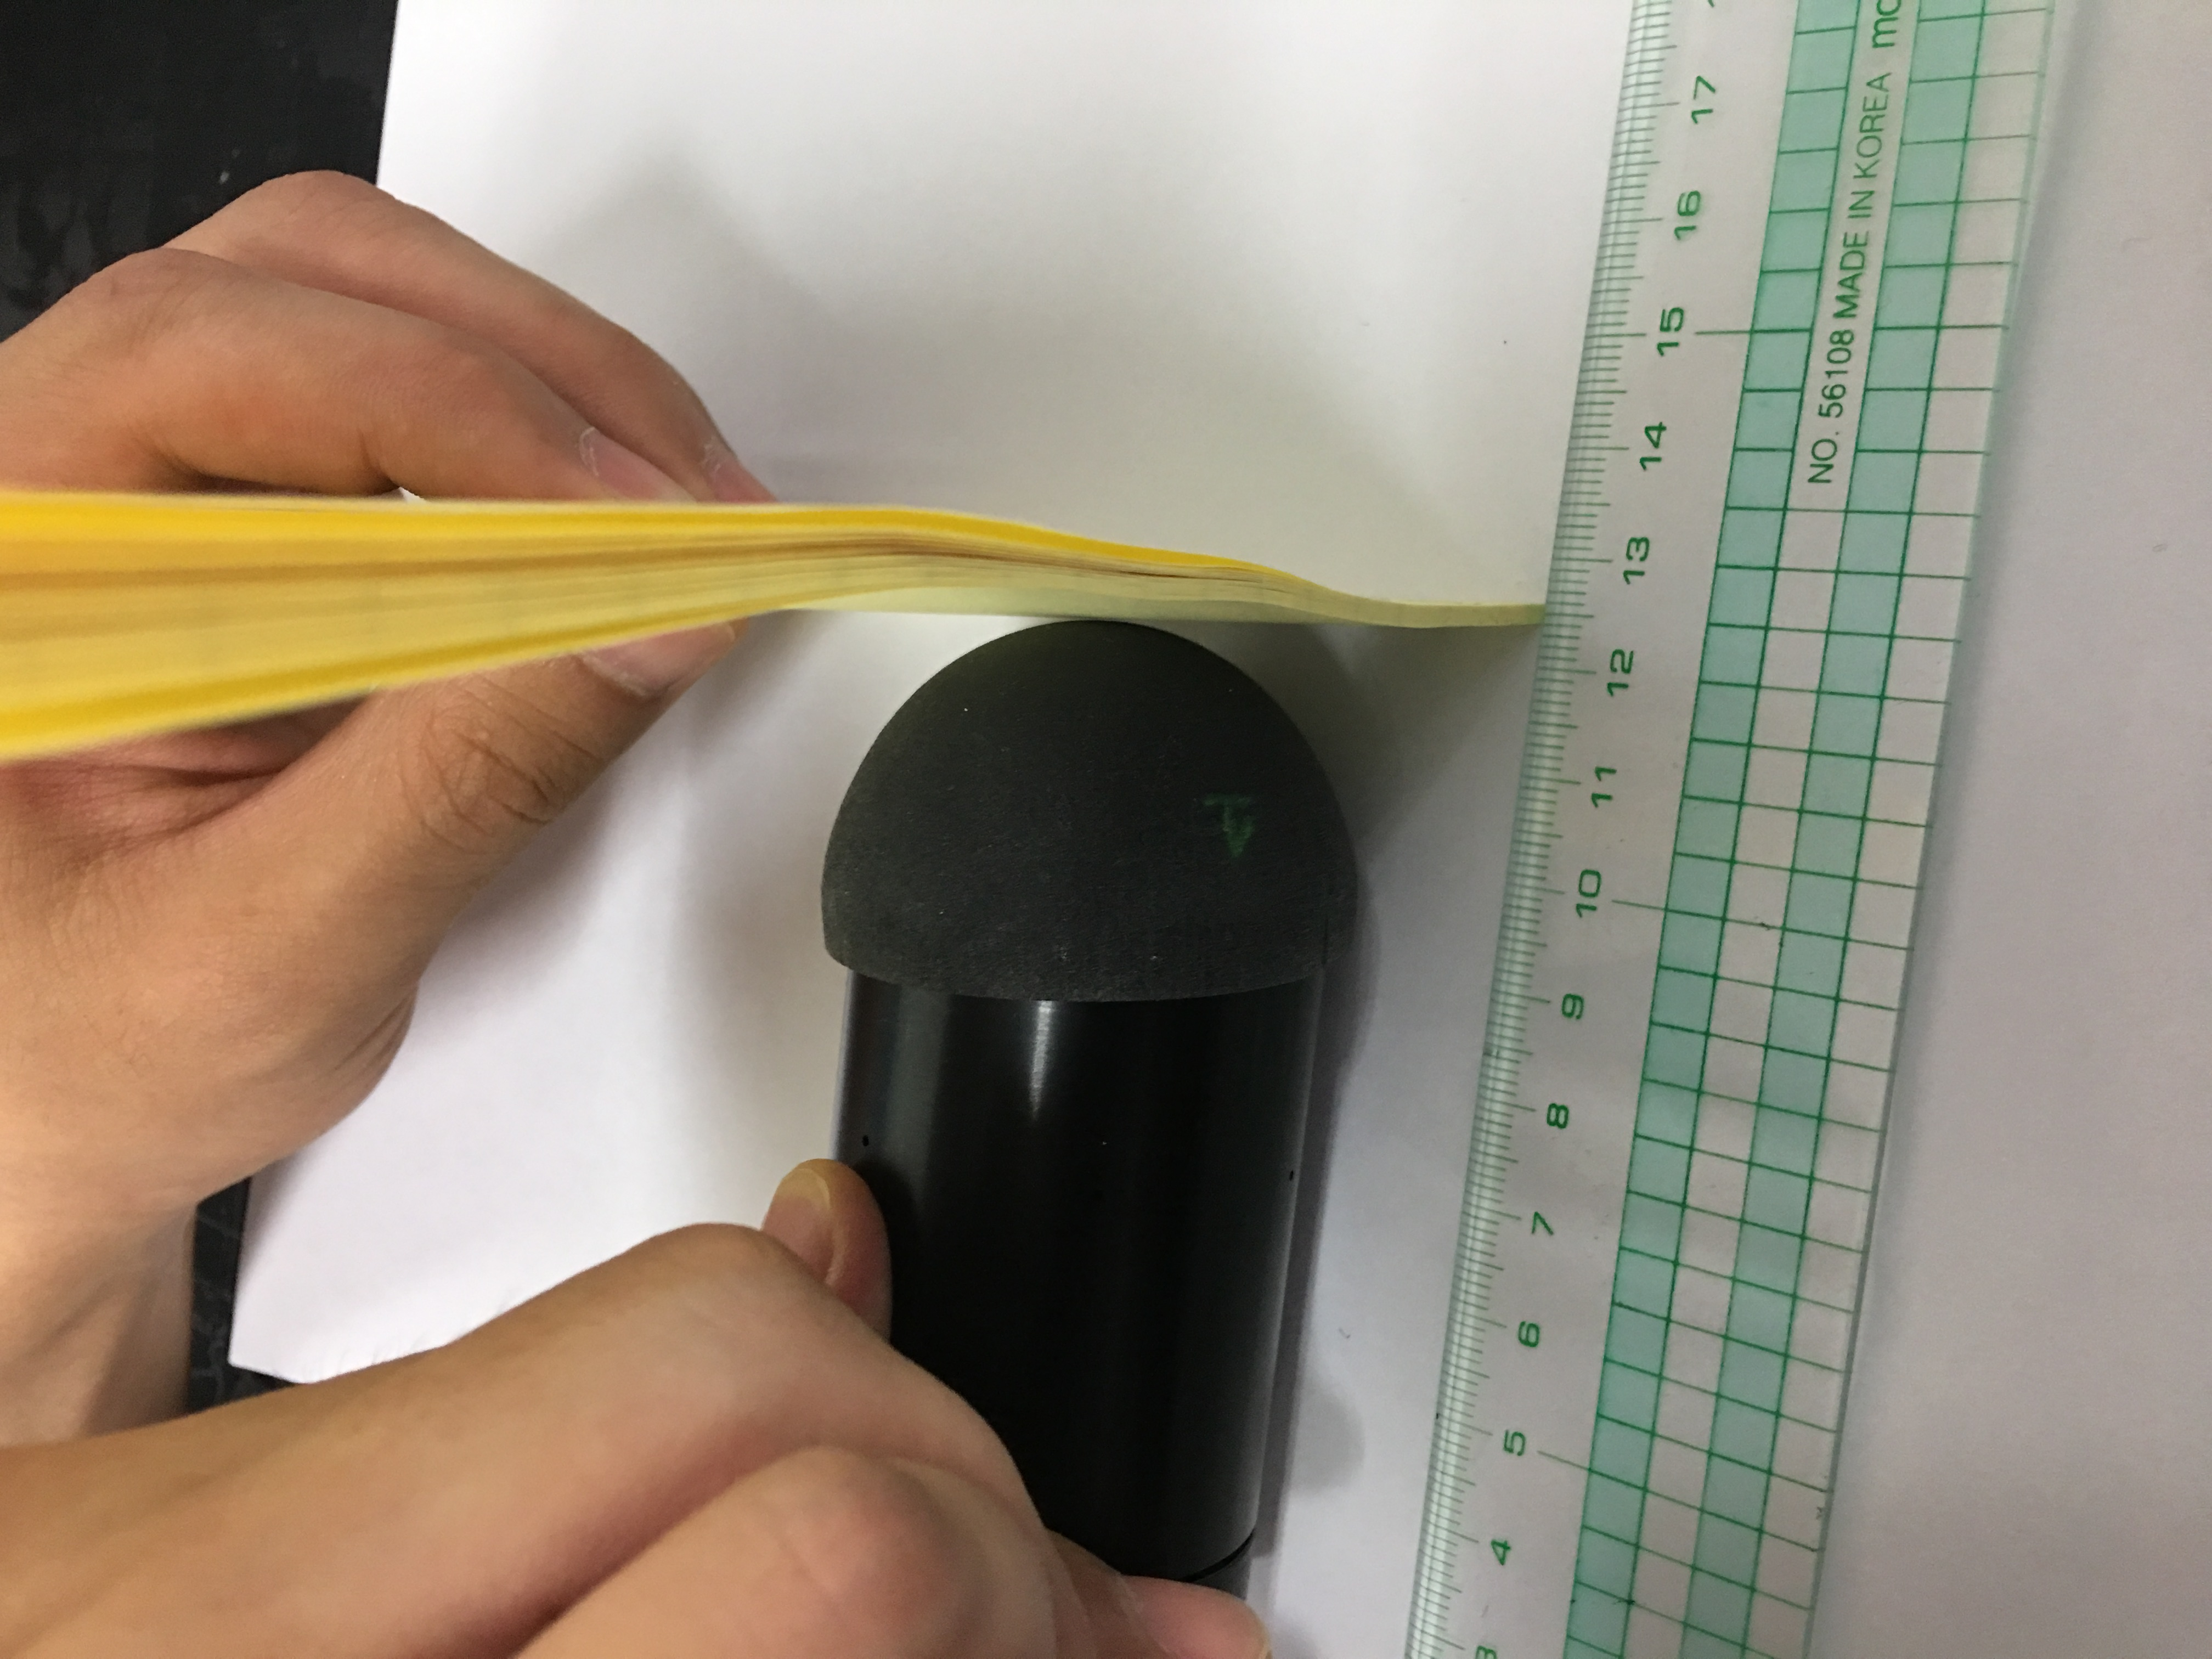
\includegraphics[width=0.3\textwidth]{img03.jpg}}
\caption{촉각센서 이미지 세트 1}
\end{figure}

\begin{figure}
\centering
\ContinuedFloat
\subfloat[img01]
{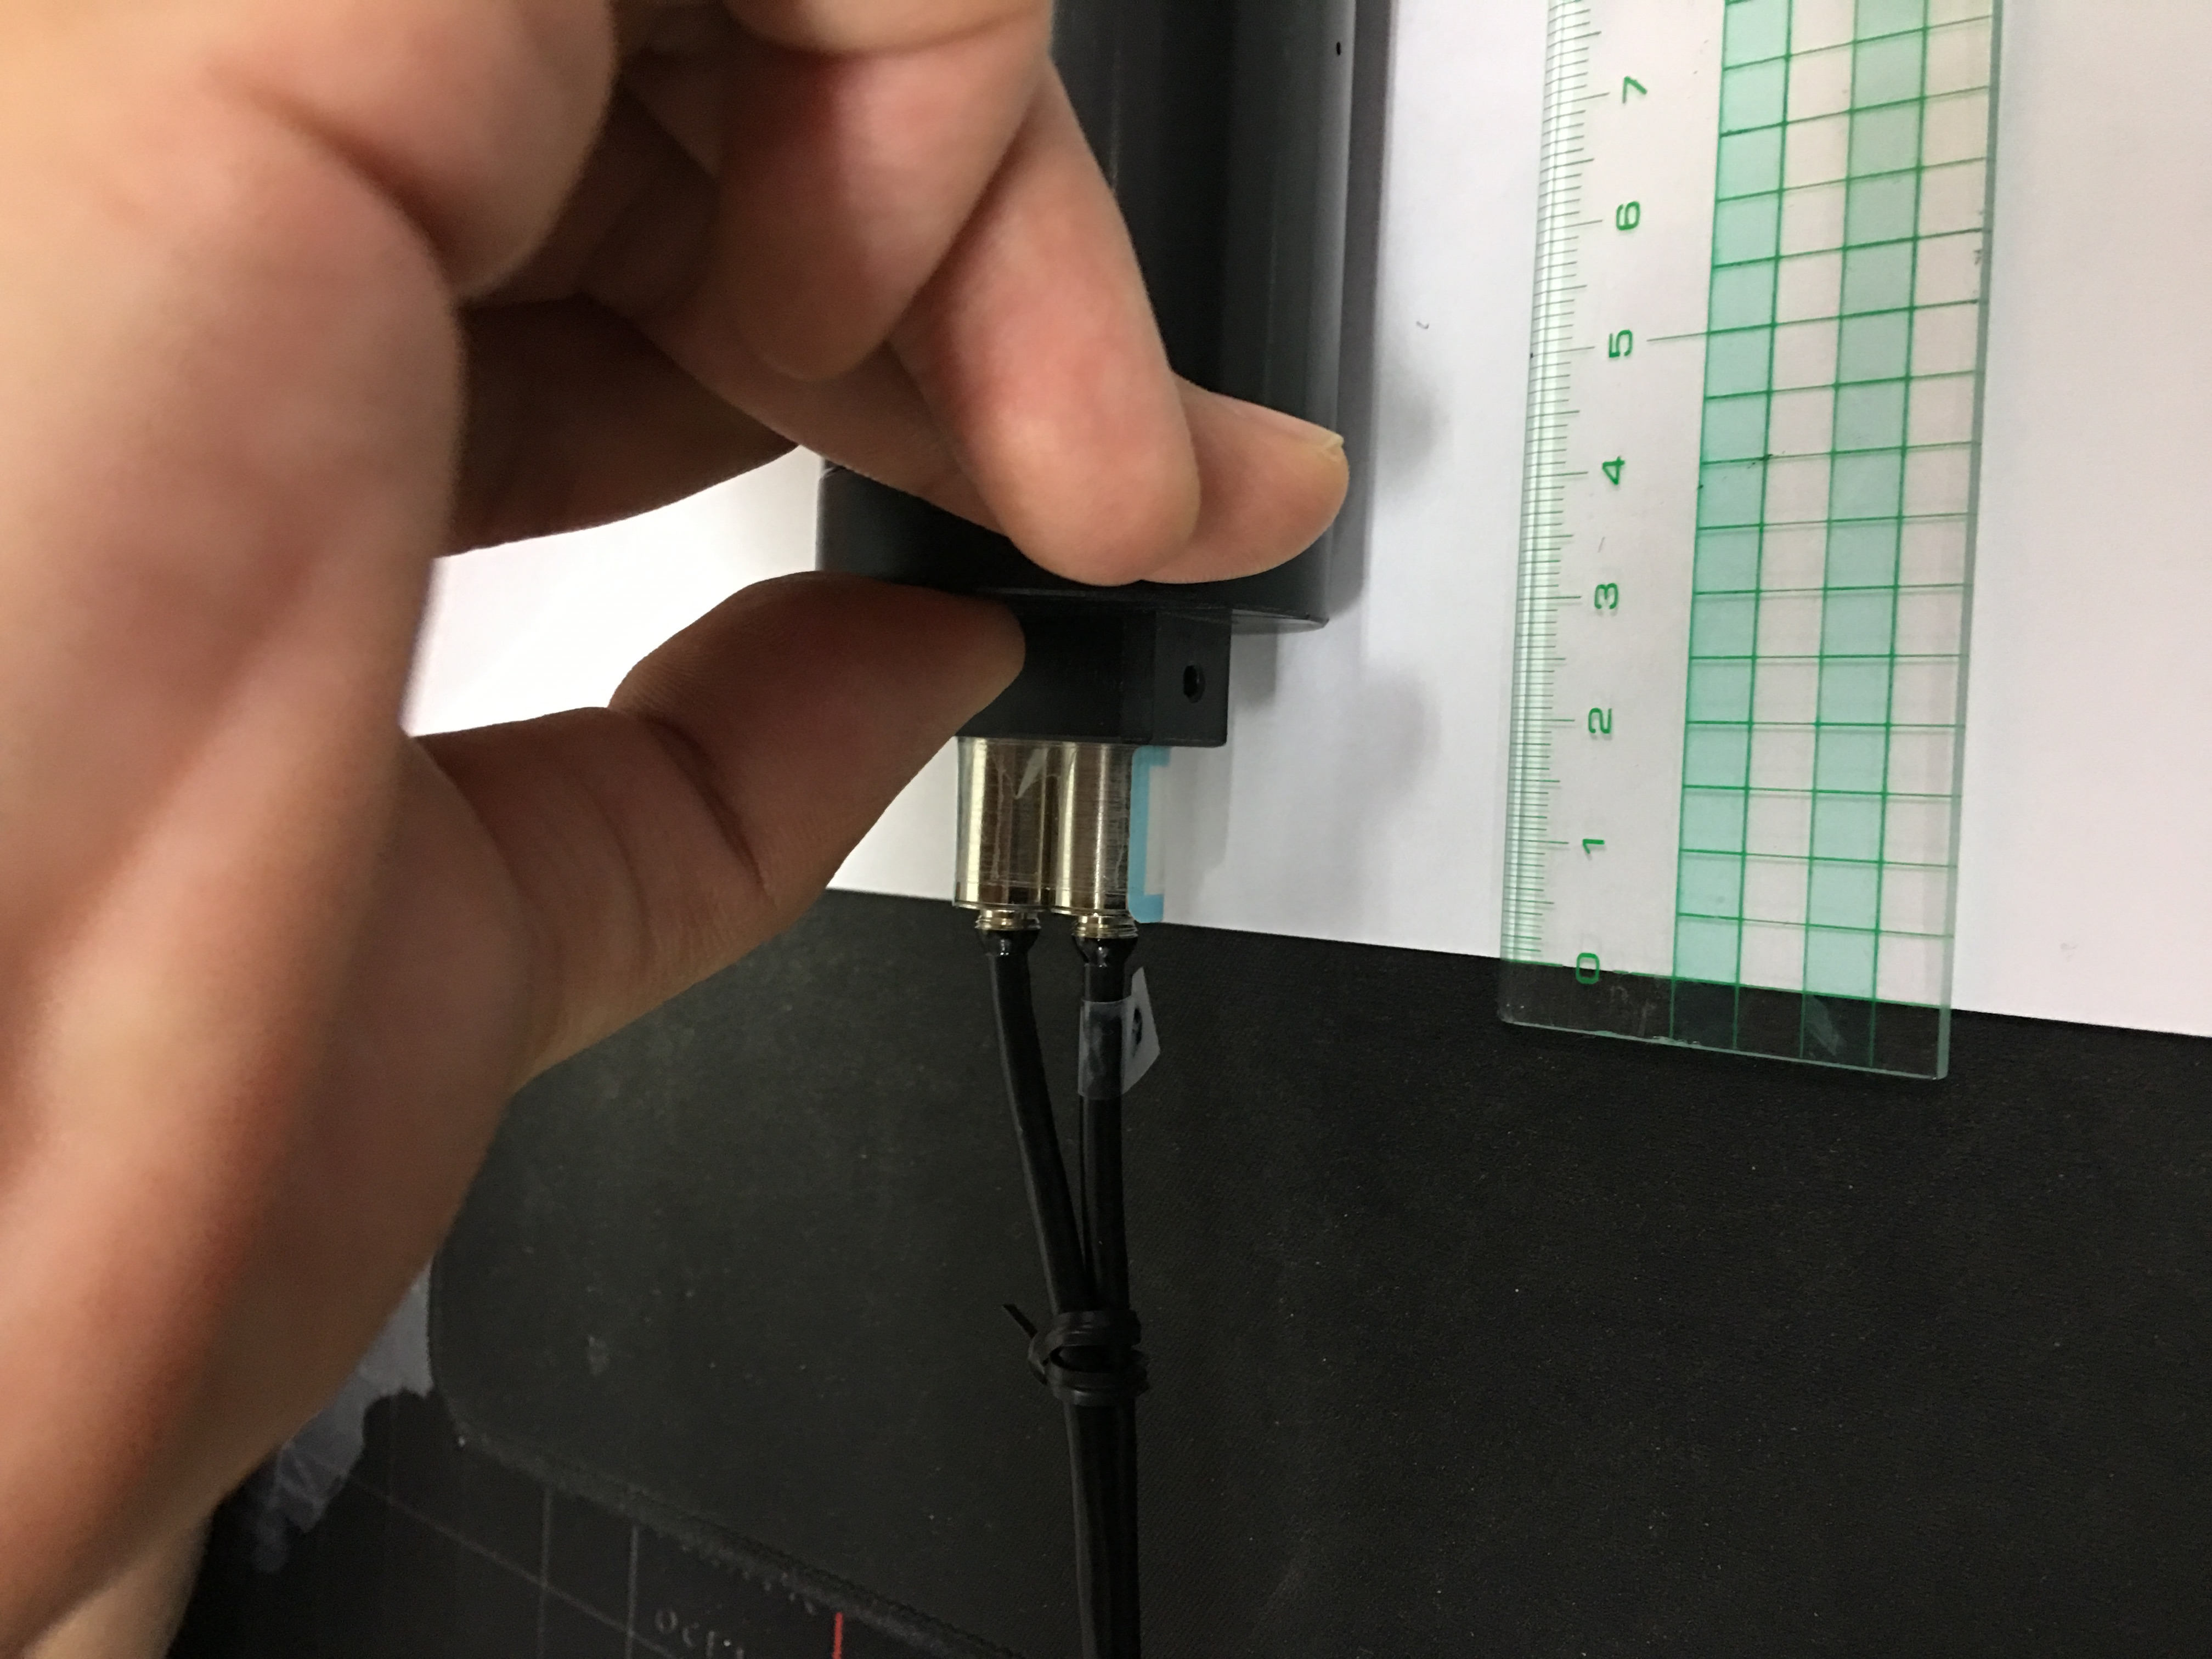
\includegraphics[width=0.3\textwidth]{img01.jpg}}
\quad
\subfloat[img02]
{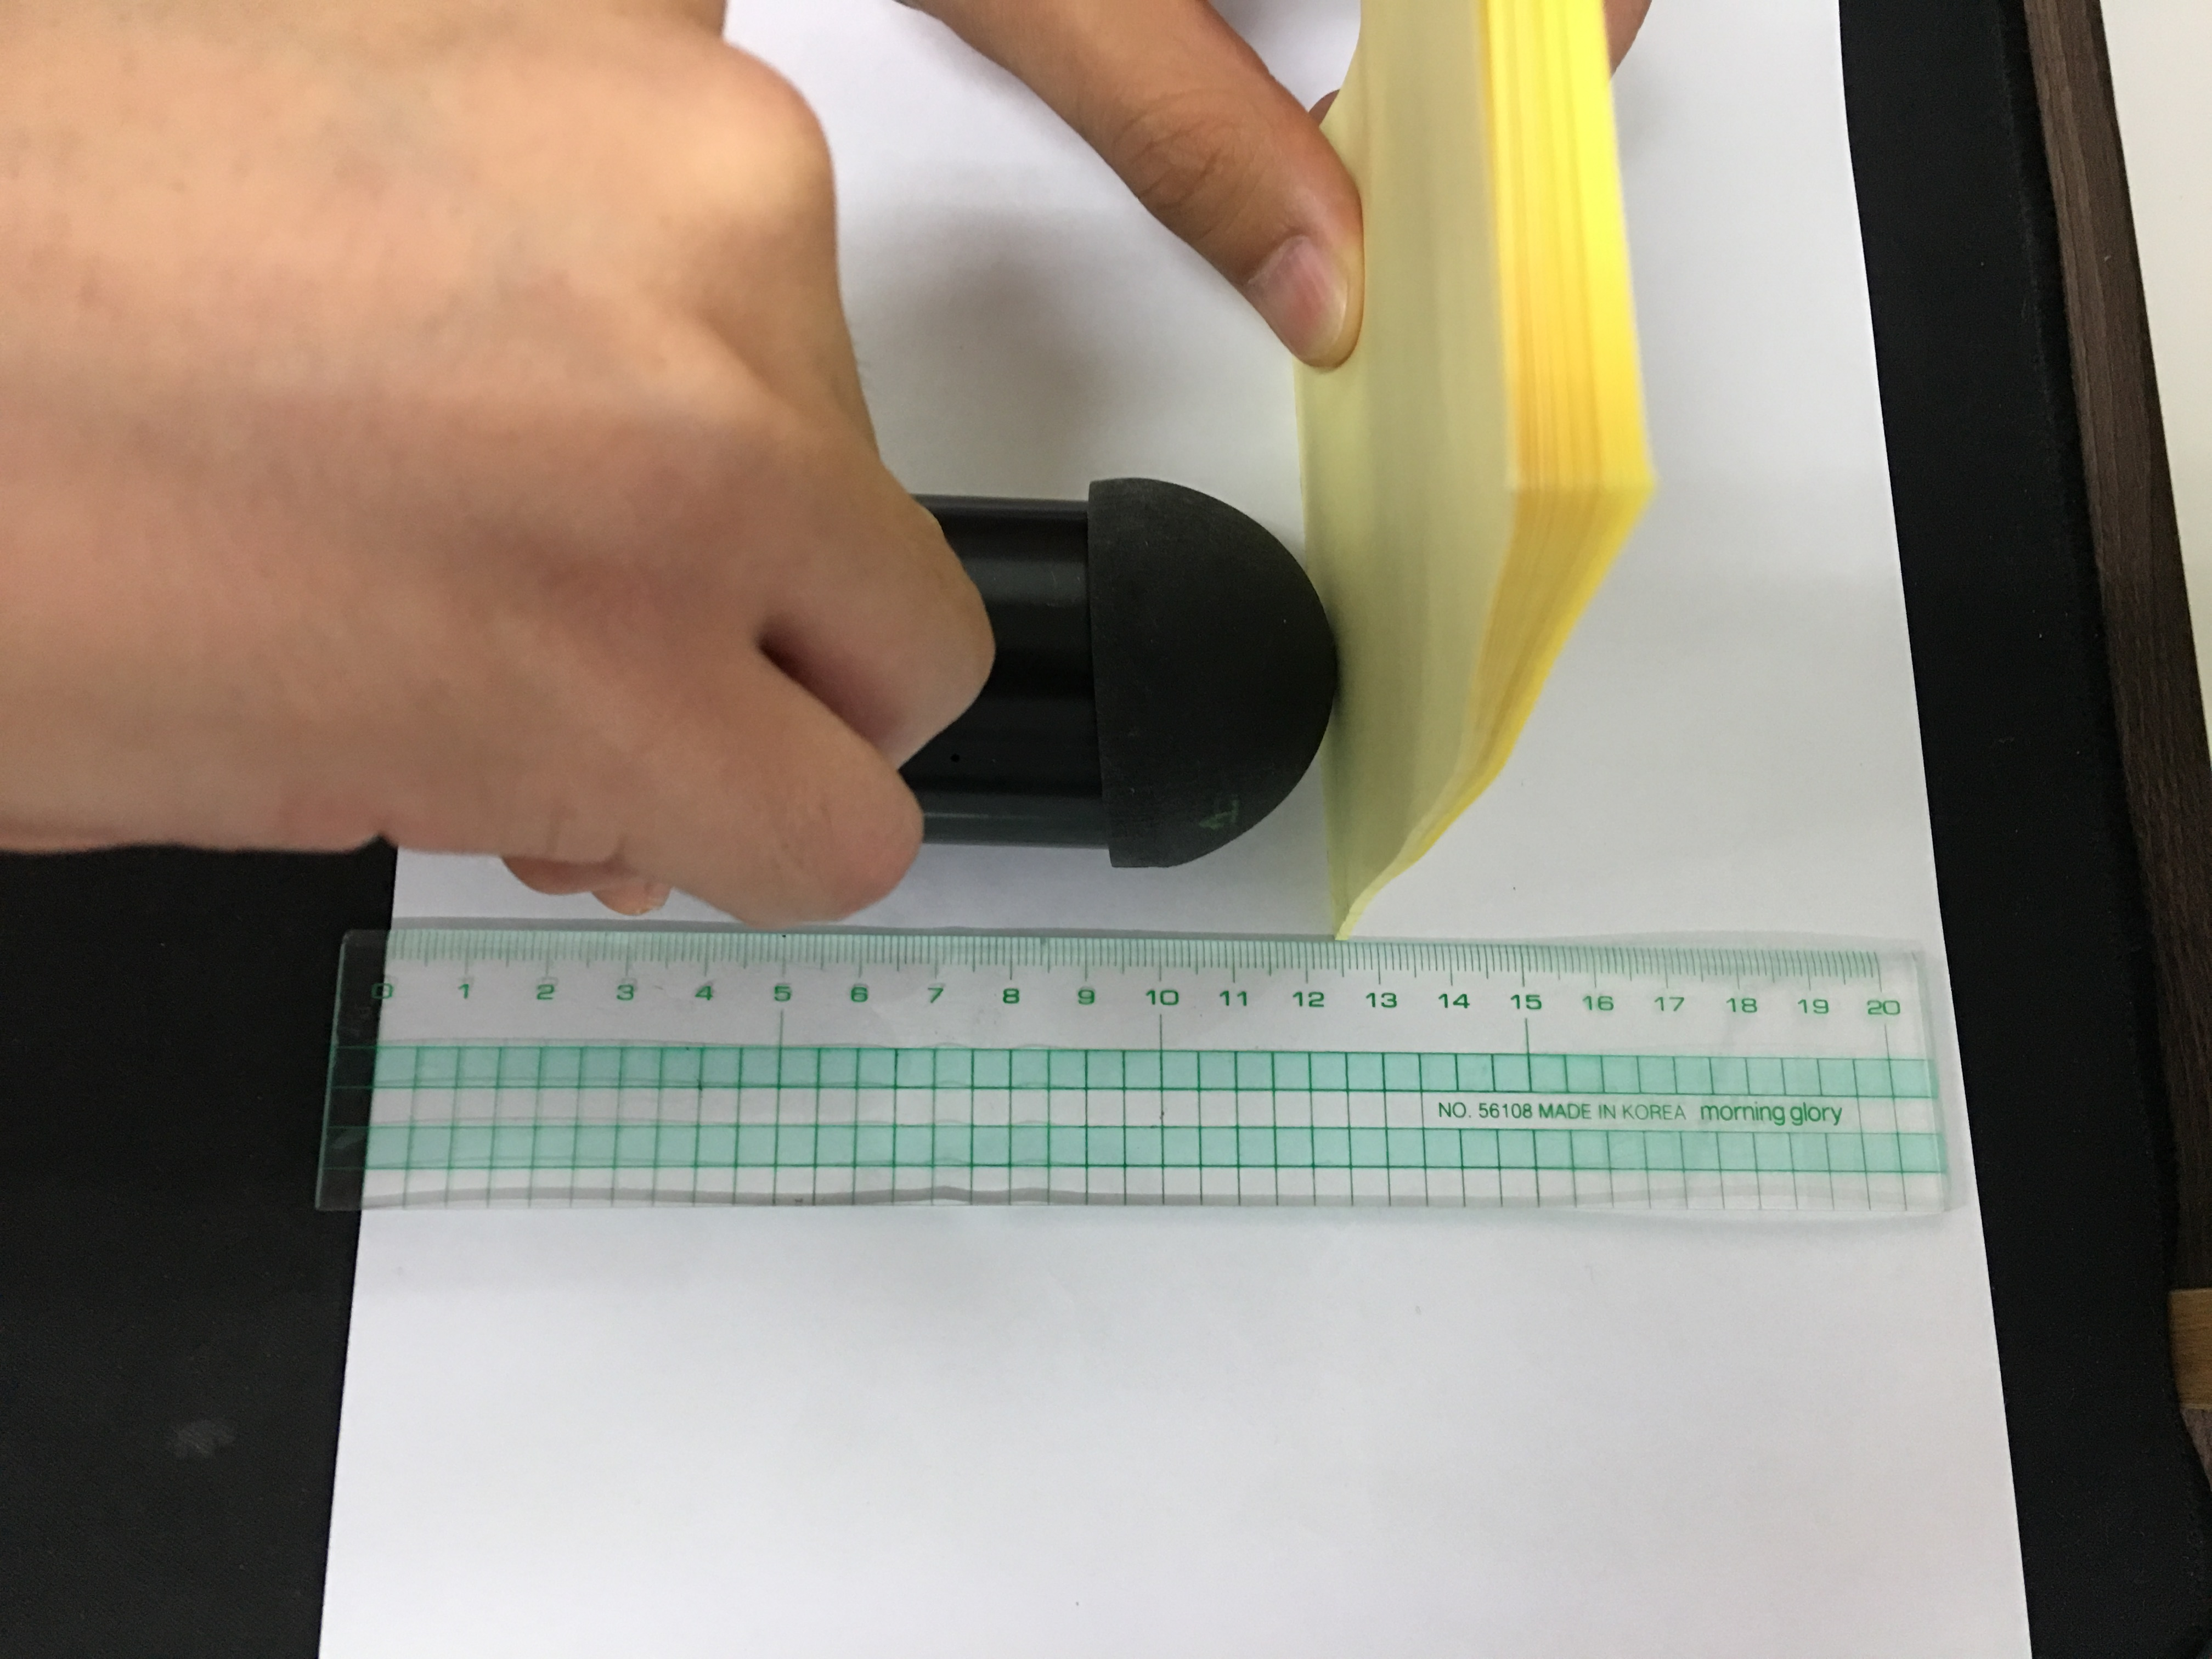
\includegraphics[width=0.3\textwidth]{img02.jpg}}
\quad
\subfloat[img03]
{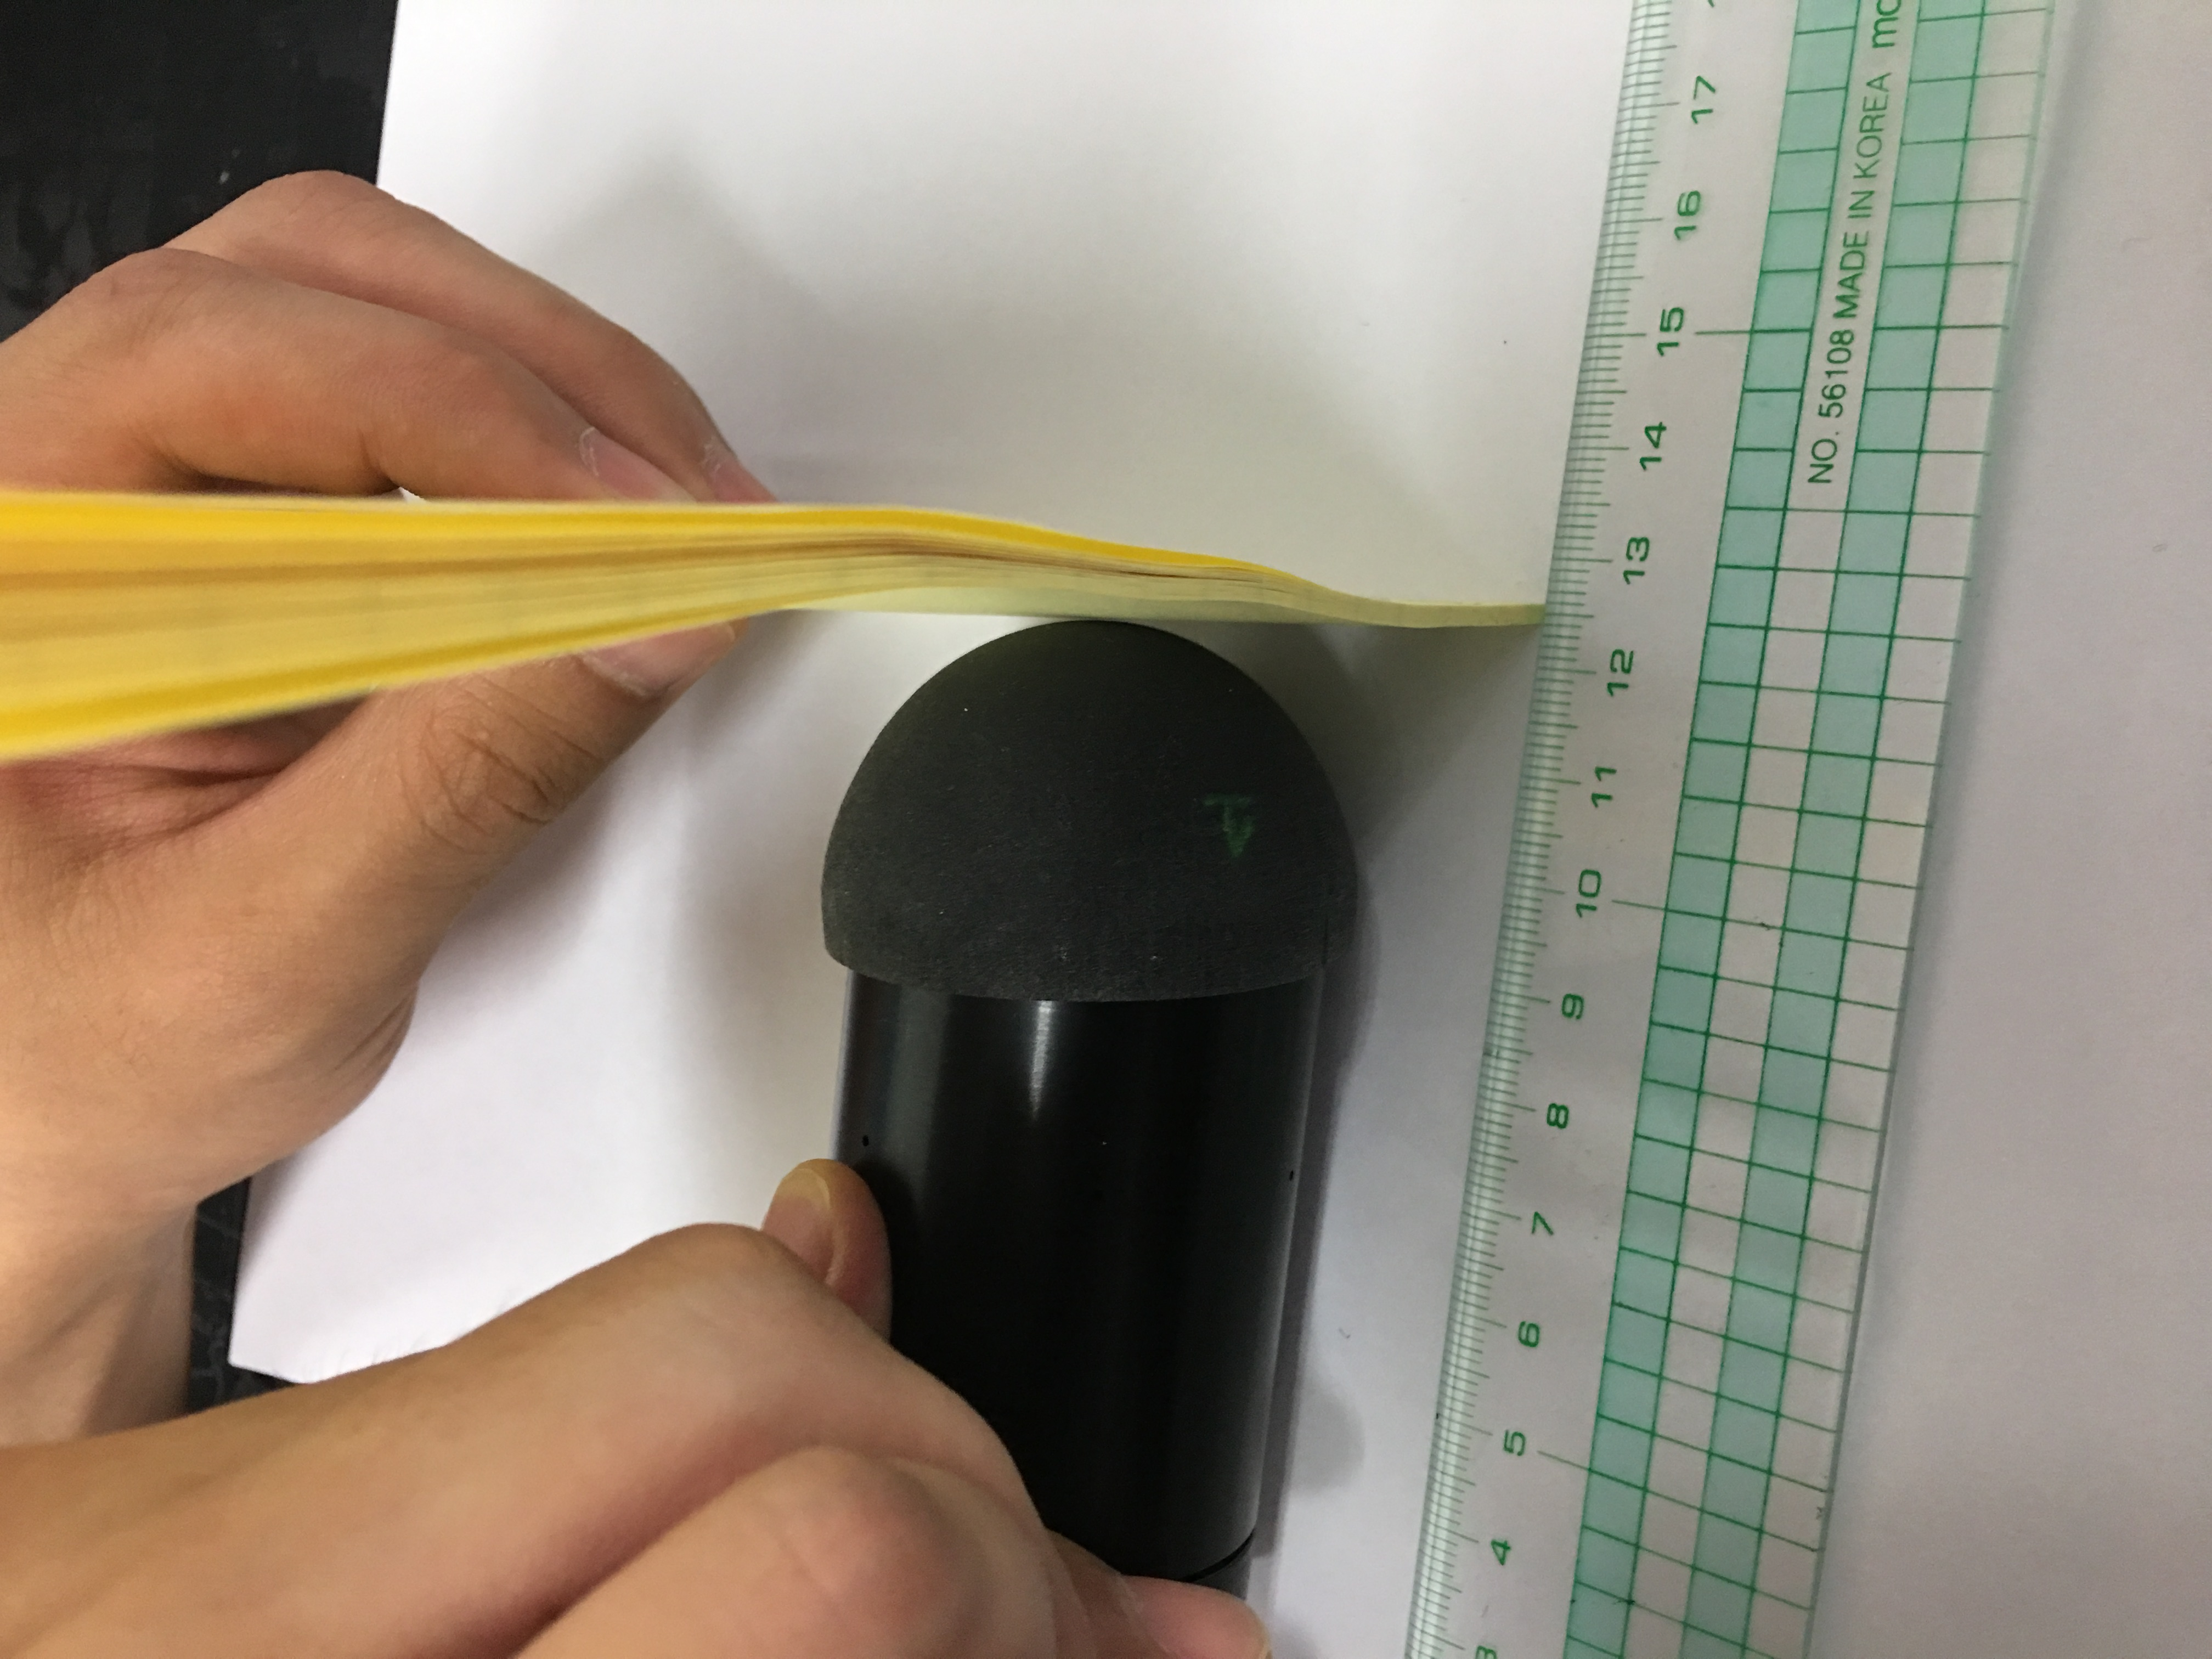
\includegraphics[width=0.3\textwidth]{img03.jpg}}
\caption{촉각센서 이미지 세트 1}
\end{figure}

\begin{tabu}spread 10pt
	{|X|[2pt, OliveDrab] X|[5pt,Plum] X|[10pt, RedViolet]}
	탄한 녹색 & 자두색 & 붉은 빛 오렌지
\end{tabu}

\begin{tabu} to 0.4\textwidth {X[c] | X[c]}
\hline
\multirow{5}{*}{레드벨벳} 
&아이린\\ \tabucline{2}
&슬기\\ \tabucline{2}
&웬디\\ \tabucline{2}
&조이\\ \tabucline{2}
&예리\\ \hline
\end{tabu}

\small
\begin{tabu}{ X[0.7,c] | X[1.4,c] | X[1.2,c] | X[1,c] | X[1,c] | X[0.7,c] | X[0.5,c] }
& 더불어민주당 & 자유한국당 & 국민의당 & 바른정당 & 정의당 & 기타 \\ \hline
의석수 & & & & & &
\end{tabu}

\end{document}